\documentclass{article}
\usepackage[utf8]{inputenc}
\usepackage[T1]{fontenc}
\usepackage{amsmath}
\usepackage{amssymb}
\usepackage{tikz}
\usepackage{hyperref}
\hypersetup{
	colorlinks=true,
	linkcolor=blue
}

\title{Digital signature}
\author{}
\date{2021-05-11}

\begin{document}

	\maketitle

	\section{Digital signature}

	A \emph{digital signature} is a piece of information (i.e. a sequence of
	bits) attached to a message which provides the three following properties:
	\begin{itemize}
		\item \textbf{Message authentication} - the receiver of the message can
			verify the origin of the message
		\item \textbf{Message integrity} - if the message gets modified the
			receiver is able to detect it
		\item \textbf{Non repudiation} - the signer cannot later claim that he
			or she didn't sign it\footnote{Actually, to gain non-repudiation 
			we also need a public key certificate, but we won't explore 
			technical details in this paper, and we'll suppose that the key
			used to sign is unequivocally linked to the signer.}.
	\end{itemize}

	\subsection{Digital signature scheme}

	A digital signature scheme consists of the following three probabilistic
	algorithms:

	\begin{itemize}
		\item \texttt{Gen(n)} - generate a symmetric key pair \texttt{(pk, sk)}
			of \texttt{n} bits, where \texttt{n} is a security parameter.
		\item $\texttt{Sign}_{\texttt{sk}}\texttt{(m)}$ - generate a digital
			signature $\sigma$ from the \emph{secret key} \texttt{sk} and the
			\emph{message} \texttt{m}.
		\item $\texttt{Vrfy}_{\texttt{pk}}\texttt{(m,}\sigma\texttt{)}$ - input
			\texttt{pk}, \texttt{m} and $\sigma$, output
			1 if the signature is valid, 0 if the signature is invalid.
	\end{itemize}

	It's  important to notice that while the key \texttt{pk} is public and
	available to everyone, the secret key \texttt{sk} must be kept, indeed,
	secret.

	\subsubsection{Security of the digital signature scheme}

	A digital signature scheme \texttt{(Gen, Sign, Vrfy)} is
	\hypertarget{security}{\emph{secure}}
	if an adversary knowing \texttt{pk} and other valid signatures $(m_{1},
	\sigma_{1}), (m_{2}, \sigma_{2}), \dots$ is not able to produce a new
	message $m$ and a valid signature $\sigma$ for it.

	\paragraph{Exercise 10.2.1}
	
	What is the difference between a MAC and a digital signature?

	\begin{itemize}
		\item MAC guarantees only authentication and integrity, while digital
			signature (in principle) also guarantees non-repudiation.
		\item A digital signature is created with a key pair \texttt{(pk, sk)},
			while the MAC is based on a secret key, shared between the sender
			and the receiver.
	\end{itemize}

	\subsection{Digital signature protocol}

	Let's consider a sender and a receiver (Alice and Bob).

	Alice wants to send a message $m$ to Bob by using her secret key
	$\texttt{sk}_{\texttt{A}}$. 

	Bob knows Alice's public key (which is indeed public) and is able to verify
	the signature.
	
	\begin{center}
		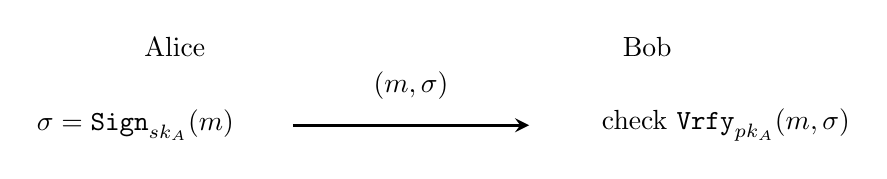
\begin{tikzpicture}[>=stealth]
			\node at (0, 1) {Alice};	
			\node at (3, .5) {$(m, \sigma)$};
			\draw[->,very thick] (1.5, 0) -- (4.5, 0);
			\node at (6, 1) {Bob};
			\node at (-.5, 0) {$\sigma = \texttt{Sign}_{sk_{A}}(m)$};
			\node at (7, 0) {$\text{check} ~ \texttt{Vrfy}_{pk_{A}}(m, \sigma)$};
		\end{tikzpicture}
	\end{center}

	\paragraph{Properties:}

	\begin{itemize}
		\item The signature is \emph{authentic} - Bob knows that Alice signed the
			message.
		\item The signature is \emph{unforgeable} - only Alice knows her private
			key.
		\item The signature is \emph{not reusable} for any other message -
			because it's a function of the message.
		\item Any \emph{alteration} of the message would invalid the signature -
			it won't be possible to verify the signature with Alice's public key anymore.
		\item The signature cannot be \emph{repudiated} - Alice cannot claim not
			having signed the message because she was the only one knowing her
			private key.
	\end{itemize}

	\subsection{Digital signature and timestamp}

	Digital signatures should also include timestamps (attach a timestamp to the
	message and sign the whole document). 

	Let's consider the following \emph{example}, taken from the Bruce Schneier's book
	“Applied Cryptography”:
	\begin{quotation}
		Alice sends Bob a signed digital check for \$100. Bob takes the check to
		the bank, which verifies the signature and moves the money from one
		account to another.
		The following week, Bob takes the same check to the bank, which again
		verifies the signature and moves the money from one account to another.
		And so on.

		But if date and time of signature are attached to the message, then the bank
		could store this timestamp into a database, and when Bob takes the check for
		the second time, the bank checks the timestamp against its database.
	\end{quotation}

	\subsection{RSA digital signature}

	\subsubsection{Naive RSA-signature}

	Alice's public key $\texttt{pk}_{A} = (n, e)$ and secret key is
	$\texttt{sk}_{A} = d$.

	\begin{center}
		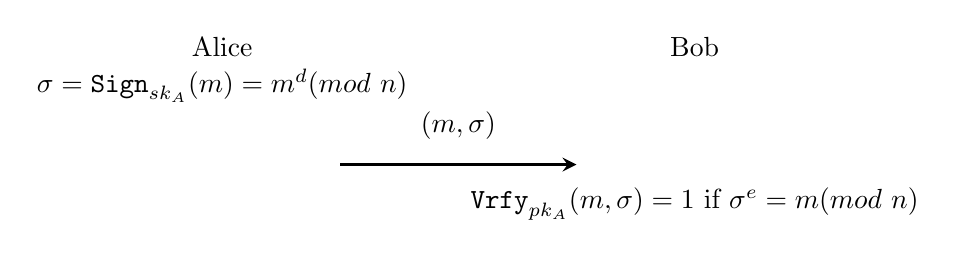
\begin{tikzpicture}[>=stealth]
			\node at (0, 1) {Alice};	
			\node at (3, 0) {$(m, \sigma)$};
			\draw[->,very thick] (1.5, -.5) -- (4.5, -.5);
			\node at (6, 1) {Bob};
			\node at (0, .5) {$\sigma = \texttt{Sign}_{sk_{A}}(m) = m^{d} (mod
			~ n)$};
			\node at (6, -1) {$\texttt{Vrfy}_{pk_{A}}(m, \sigma) = 1 ~ \text{if}
			~
			\sigma^{e} = m (mod ~ n)$};
		\end{tikzpicture}
	\end{center}

	\paragraph{Exercise 10.2.2} 

	Show that the above signature scheme is not secure.
	\emph{Hint}: choose any 
	$\sigma \in \mathbb{Z}_{n}$ and consider $m = \sigma^{e} (mod ~ n)$


	\vspace{10pt}

	First, let's remember what does it mean for a digital signature scheme
	to be \hyperlink{security}{secure}: 
	an adversary should not be able to produce a new message $m$ and a valid
	signature $\sigma$ for it. 

	Now, let's pick $\sigma \in \mathbb{Z}^{*}_{n}$. We define $m := \sigma^{e}
	(mod ~ n)$.
	Then it is true that:
	$$
		m = \sigma^{e} (mod ~ n) \quad \Longrightarrow \quad \sigma^{e} = m (mod ~ n)
	$$
	
	But this means that, by definition of our scheme,
	$\texttt{Vrfy}_{\texttt{pk}_{A}} (m, \sigma) = 1$, and therefore $\sigma$ is
	a valid signature for $m$.

	Now, some might argue that this isn't a realistic attack because the adversary 
	has not control over $m$. Actually this is irrelevant to our purposes: plain
	RSA signature doesn't respect digital signature security requisites.

	\subsection{EMSA-PSS - RSA digital signature}


	\emph{Encoding method for signature with appendix probabilistic signature
	scheme.} 
	(see also \url{https://tools.ietf.org/rfc/rfc3447.txt}).
	
	\renewcommand{\labelitemi}{-}

	The following method is parametrized by the choice of:
	\begin{itemize}
		\item Hash function 
		\item Mask generation function
		\item Salt length
	\end{itemize}

	\begin{center}
		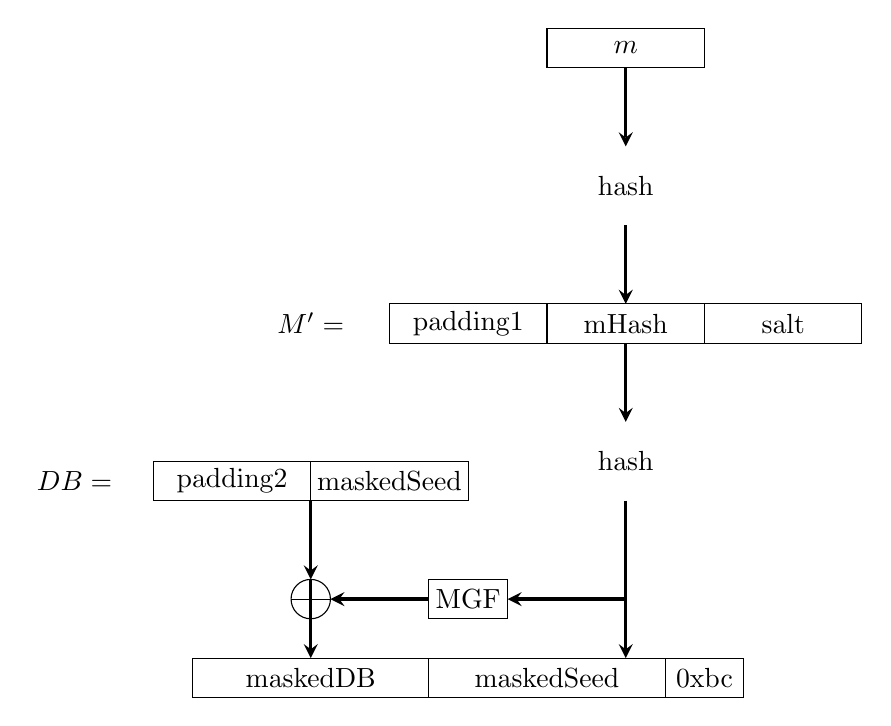
\begin{tikzpicture}[>=stealth]
			\draw (3, 6) rectangle +(2, .5);
			\node at (4, 6.25) {$m$};
			\draw[->,very thick] (4, 6) -- +(0, -1);
			\node at (4, 4.5) {hash};
			\draw[->,very thick] (4, 4) -- +(0, -1);
			\node at (0, 2.75) {$M' =$};
			\draw (1, 2.5) rectangle +(2, .5) node[pos=.5] {padding1};
			\draw (3, 2.5) rectangle +(2, .5) node[pos=.5] {mHash};
			\draw (5, 2.5) rectangle +(2, .5) node[pos=.5] {salt};
			\draw[->,very thick] (4, 2.5) -- +(0, -1);
			\node at (4, 1) {hash};
			\draw[->,very thick] (4, .5) -- +(0, -2);
			\node at (-3, .75) {$DB=$};
			\draw (-2, .5) rectangle +(2, .5) node[pos=.5] {padding2};
			\draw (0, .5) rectangle +(2, .5) node[pos=.5] {maskedSeed};
			\draw[->,very thick] (0, .5) -- +(0, -1);
			\draw[->,very thick] (4, -.75) -- +(-1.5, 0);
			\draw (1.5, -1) rectangle +(1, .5) node[pos=.5] {MGF};
			\draw[->,very thick] (1.5, -.75) -- +(-1.25, 0);
			\draw (0, -.75) circle (.25);
			\draw (-.25, -.75) -- +(.5, 0);
			\draw (0, -.5) -- +(0, -.5);
			\draw[->,very thick] (0, -.5) -- +(0, -1);
			\draw (-1.5, -2) rectangle +(3, .5) node[pos=.5] {maskedDB};
			\draw (1.5, -2) rectangle +(3, .5) node[pos=.5] {maskedSeed};
			\draw (4.5, -2) rectangle +(1, .5) node[pos=.5] {0xbc};
		\end{tikzpicture}
	\end{center}






\end{document}
